\documentclass[CJK, 10pt]{beamer}
\usepackage{CJKutf8}
\usepackage{graphicx}
\usepackage{xcolor}
\usepackage{hyperref}
\hypersetup{
  urlcolor=blue,
  colorlinks=true,
  linkcolor=blue,
  bookmarks=false,
}

\usetheme{Boadilla}
\setbeamercovered{transparent}

\AtBeginSection[]
{
    \begin{frame}
        \tableofcontents[currentsection,hideallsubsections]
    \end{frame}
}
\AtBeginSubsection[]
{
    \begin{frame}[shrink]
        \tableofcontents[sectionstyle=show/shaded,subsectionstyle=show/shaded/hide]
    \end{frame}
}

\setbeamerfont{block body}{size=\scriptsize}

\begin{document}
\begin{CJK*}{UTF8}{gbsn}

\title{Git原理与实践}
\author{youngsterxyf}
\institute{众成技术聚乐部}
\date{}

\begin{frame}[plain]
	\titlepage
\end{frame}

\section*{大纲}
\begin{frame}
\tableofcontents
\end{frame}

%%%%%%%%%%%%%%%%%%%%%%%%%%%%%%%%
\section{简介}
\begin{frame}{背景}
    \begin{block}{Linux内核版本管理}
    \begin{itemize}
        \item 2002 \textendash\ 2005: BitKeeper
        \item 2005 \textendash\ : $\rightarrow$ Git
    \end{itemize}
    \end{block}
    \begin{block}{Git的设计目标}
    \begin{itemize}
    	\item 速度
    	\item 简单的设计
    	\item 对非线性开发模式的强力支持(允许上千个并行开发的分支)
    	\item 完全分布式
    	\item 有能力高效管理类似Linux内核一样的超大规模项目(速度和数据量)
    \end{itemize}
    \end{block}
\end{frame}
\begin{frame}{与SVN的区别}
    \begin{block}{}
        \begin{itemize}
                \item 分布式
                \item 直接记录快照,而非差异比较
                \item 分支模型
                \item 权限管理
                \item ...
            \end{itemize}
    \end{block}
\end{frame}

\section{实践(上)}
\begin{frame}{基本用法}
    \begin{block}{新建代码库}
        \begin{enumerate}
            \item git init
            \item git add *
            \item git commit -m 'bbb'
            \item git remote add origin http://xxx.yyy
            \item git push origin master
        \end{enumerate}
    \end{block}
    \begin{block}{变更提交}
        \begin{enumerate}
            \item git add xxx / git rm yyy / git mv xxx yyy
            \item git commit -m 'aaa'
            \item git push origin master
        \end{enumerate}
    \end{block}
    \begin{block}{更新代码}
        \begin{enumerate}
            \item git fetch origin master
            \item git merge origin/master
        \end{enumerate}
        或合并为
        \begin{itemize}
            \item git pull origin master
        \end{itemize}
    \end{block}
\end{frame}
\begin{frame}{基本用法(续)}
    \begin{block}{克隆代码库}
        \begin{itemize}
            \item git clone http://xxx.yyy
        \end{itemize}
    \end{block}
    \begin{block}{分支操作}
        \begin{enumerate}
            \item git branch test /* 创建一个名为test的分支 */
            \item git checkout test /* 切换到test分支 */
            \item git push origin test /* 将test分支推送到远程服务器,即创建远程test分支 */
            \item git checkout master /* 切换回master主分支 */
            \item git branch -d$|$-D test /* 删除test分支 */
            \item git push origin :test /* 删除远程test分支 */
            \item git branch [-v] [-r] /* 查看分支列表,-v:详细信息,-r:远程分支列表 */
            \item git checkout -b local-branch origin/remote-branch /* 迁出远程分子和remote-branch到一个本地分支local-branch */
        \end{enumerate}
        步骤1、2可合并为:
        \begin{itemize}
            \item git checkout -b test /* 创建一个名为test的分支,并切换到该分支 */
        \end{itemize}
        步骤8实际可分为两个步骤:
        \begin{enumerate}
            \item git branch local-branch origin/remote-branch
            \item git checkout local-branch
        \end{enumerate}
    \end{block}
\end{frame}
\begin{frame}{基本用法(续)}
    \begin{block}{标签操作}
        \begin{itemize}
            \item git tag v0.0.1 6030bd2cc /* 在commit 6030bd2cc上打个名为v0.0.1的轻量级标签 */
            \item git tag -a v0.0.1 -m 'xxx' /* 在当前HEAD指向的commit上打个名为v0.0.1的带附注的标签 */
            \item git show v0.0.1 /* 查看标签内容 */
            \item git push origin v0.0.1 /* 将标签推送到远程服务器 */
            \item git tag -d v0.0.1 /* 从本地仓库删除标签v0.0.1 */
            \item git push origin :v0.0.1 /* 从远程服务器删除标签v0.0.1 */
        \end{itemize}
    \end{block}
    \begin{block}{其它常用命令}
        \begin{itemize}
            \item git status /* 检查当前文件状态 */
            \item git remote -v /* 查看当前代码库所关联的远程服务器地址 */
            \item git branch -v /* 查看当前代码库有哪些分支,当前分支是哪个 */
            \item git config ... /* 配置Git */
            \item git help / git help subcommand /* 查看文档,很明显,这是最重要的命令 */
            \item git checkout * / git checkout targetfile /* 撤销未提交的变更 */
            \item git log /* 日志的输出格式可以使用一些参数进行灵活的定制 */
            \item git diff /* 不带其他选项,则显示相比暂存区,工作区的变更,另外使用不同参数,可查看不同分支、不同提交之间的差异 */
        \end{itemize}
    \end{block}
\end{frame}

%%%%%%%%%%%%%%%%%%%%%%%%%%%%%%%%
\section{原理}
\begin{frame}{基本操作流程}
    \begin{center}
        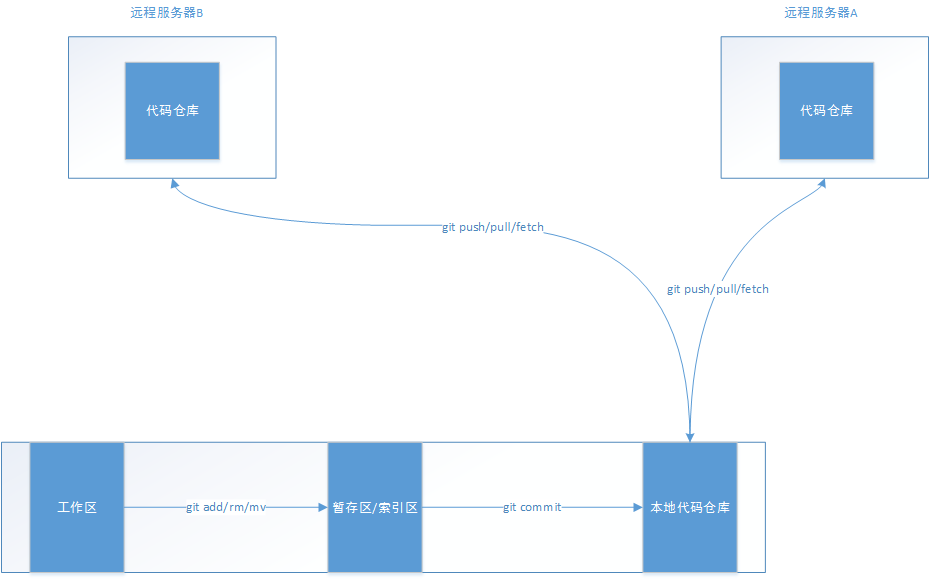
\includegraphics[width=10cm]{git-basic-process.png}
    \end{center}
\end{frame}

\begin{frame}{存储模型}
    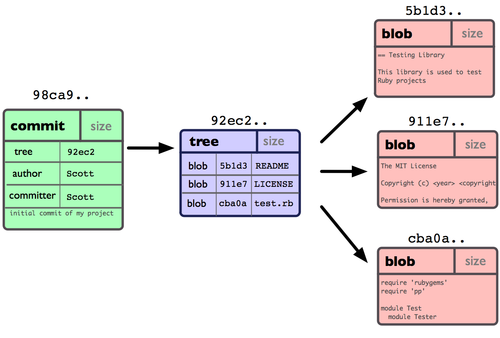
\includegraphics[width=5cm]{commit-ds.png} \hfill 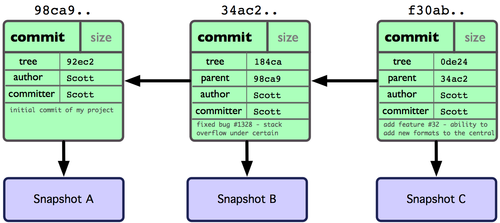
\includegraphics[width=5cm]{commit-links.png}
\end{frame}

\begin{frame}{存储模型(续)}
    \begin{block}{}
        Git以一种类似UNIX文件系统但更简单的方式来存储内容。所有内容以tree或blob对象存储,其中tree对象对应于UNIX中的目录,blob对象则大致对应于inodes或文件内容。
        一个单独的tree对象包含一条或多条tree记录,每一条记录含有一个指向blob或子tree对象的SHA-1指针,并附有该对象的权限模式(mode)、类型和文件名信息。
    \end{block}
    \begin{block}{}
        commit 对象有格式很简单:指明了该时间点项目快照的顶层树对象、作者/提交者信息(从Git设置的user.name和user.email中获得)以及当前时间戳、一个空行,
        以及提交注释信息。
    \end{block}
    \begin{block}{对象存储}
        \begin{enumerate}
            \item Git以对象类型为起始内容构造一个文件头,然后添加一个空格,接着是数据内容的长度,最后是一个空字节(null byte)。
            \item 然后将构造出来的文件头与原始数据内容拼接起来,计算拼接后的新内容的SHA-1校验和
            \item 使用zlib对拼接后的内容进行压缩
            \item 将压缩后的内容写入磁盘,文件路径为:以SHA-1值的头两个字符作为子目录名称,剩余38个字符作为文件名保存至该子目录中
        \end{enumerate}
    \end{block}
    \begin{block}{优化}
        Git往磁盘保存对象时默认使用的格式叫松散对象(loose object)格式。Git会不定期地将这些对象打包至一个叫packfile的二进制文件以节省空间并提高效率。
        当仓库中有太多的松散对象,或是手工调用git gc命令,或推送至远程服务器时,Git都会这样做。
    \end{block}
\end{frame}

\begin{frame}{分支模型 - 分支引用}
    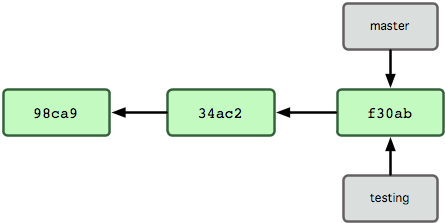
\includegraphics[width=5cm]{branch-pointer.png} \hfill 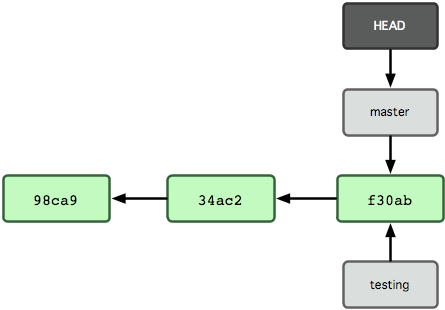
\includegraphics[width=5cm]{HEAD-point-current.png} \\
    \begin{center}
        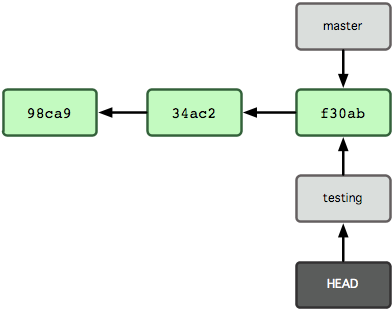
\includegraphics[width=5cm]{HEAD-point-testing.png}
    \end{center}
\end{frame}

\begin{frame}{分支模型 - 快进(Fast forward)合并}
    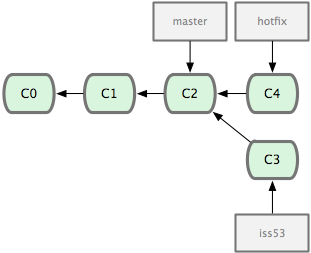
\includegraphics[width=5cm]{hotfix-branch.png} \hfill 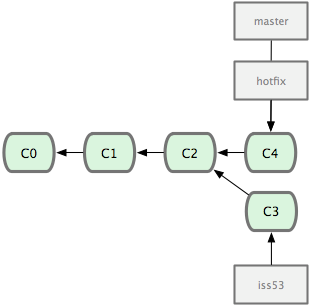
\includegraphics[width=5cm]{master-hotfix-same.png}
\end{frame}

\begin{frame}{分支模型 - 三方合并}
    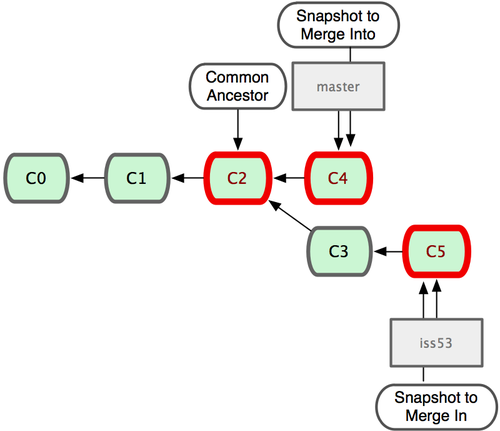
\includegraphics[width=6cm]{merge-three-part.png} \hfill 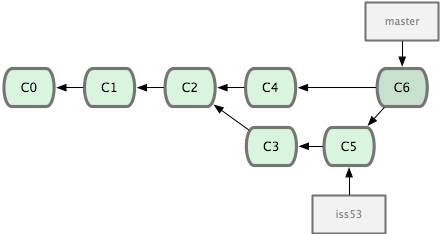
\includegraphics[width=5cm]{after-merge-three-part.png}
    \begin{block}{合并冲突}
        如果不同的分支中都修改了同一个文件的同一部分,Git自动合并就会失败,需要你进行人工合并。要看看哪些文件在合并时发生冲突,可以用git status查阅。
        在手动编辑解决了所有文件里的所有冲突后,运行git add将把它们标记为已解决状态。
    \end{block}
\end{frame}

\begin{frame}{标签}
    \begin{block}{}
        \begin{itemize}
            \item 标签(tag)与分支引用类似
            \item 标签分为两种:轻量级标签 与 含附注的标签
            \item 轻量级标签其实就是一个指向指定commit的指针
            \item 含附注的标签会有一个额外的标签对象,对象中包含“打标签的人”、“日期”、“附注”以及“指向commit的SHA-1值”
        \end{itemize}
    \end{block}
    \begin{center}
        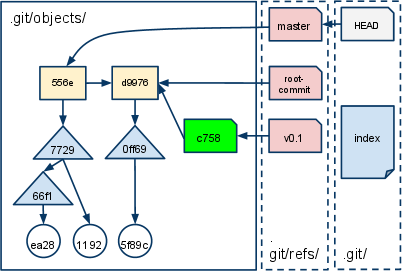
\includegraphics[width=7cm]{new-tag.png}
    \end{center}
\end{frame}

\begin{frame}{Git代码库目录结构}
.git目录即代码仓库,包含了所有数据。\\
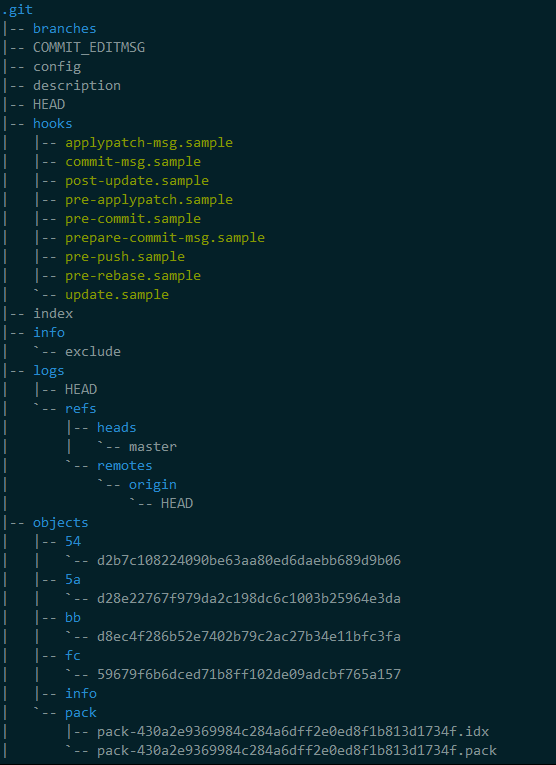
\includegraphics[width=5cm]{tree-dot-git-1.png} \hfill
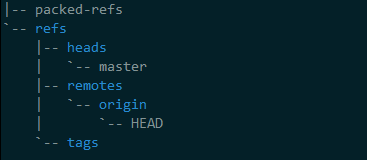
\includegraphics[width=5cm]{tree-dot-git-2.png}
\end{frame}

\begin{frame}{与远程服务器交互 - git clone}
    \begin{center}
        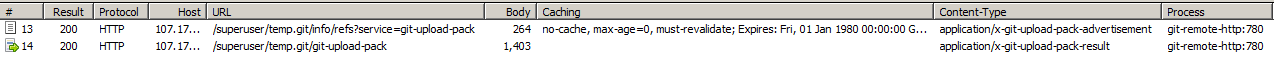
\includegraphics[width=9cm]{git-clone-remote-1.png} \\
        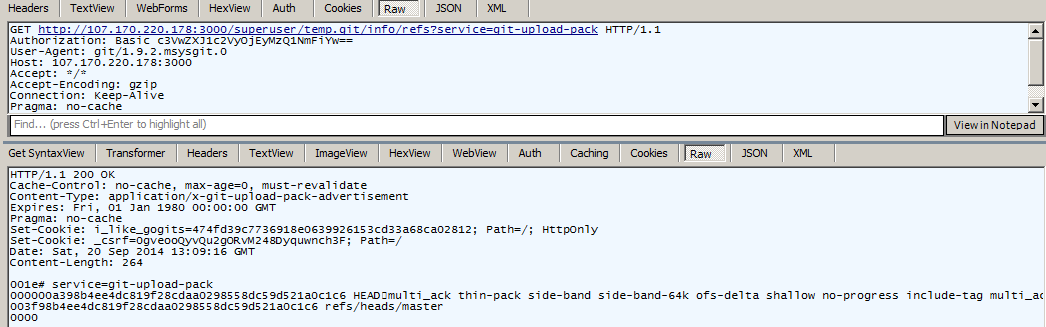
\includegraphics[width=9cm]{git-clone-remote-2.png} \\
        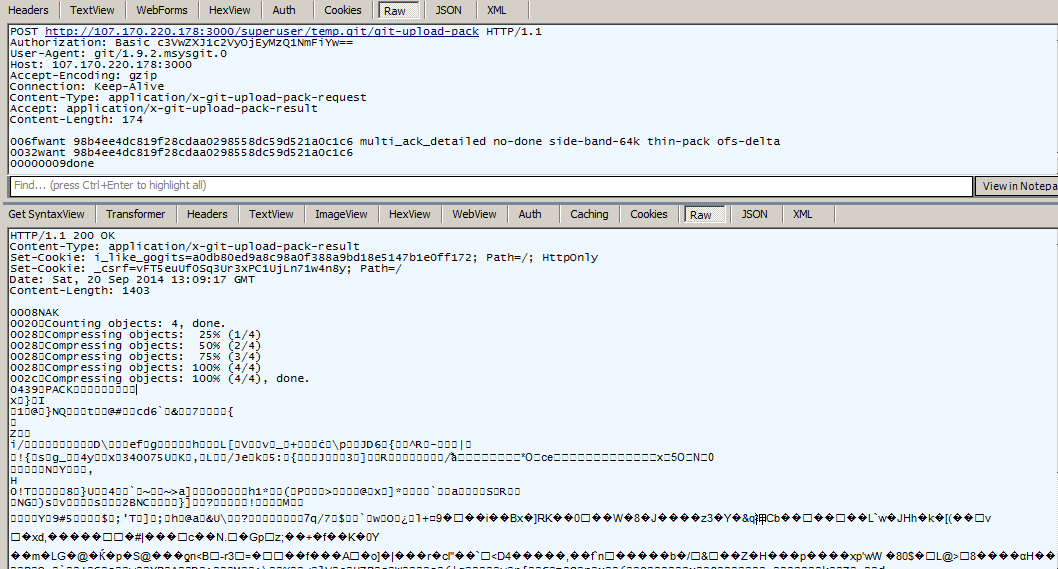
\includegraphics[width=9cm]{git-clone-remote-3.png}
    \end{center}
\end{frame}
\begin{frame}{与远程服务器交互 - git push}
    \begin{center}
        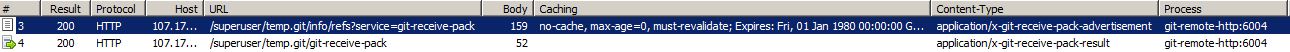
\includegraphics[width=10cm]{git-push-remote-1.png} \\
        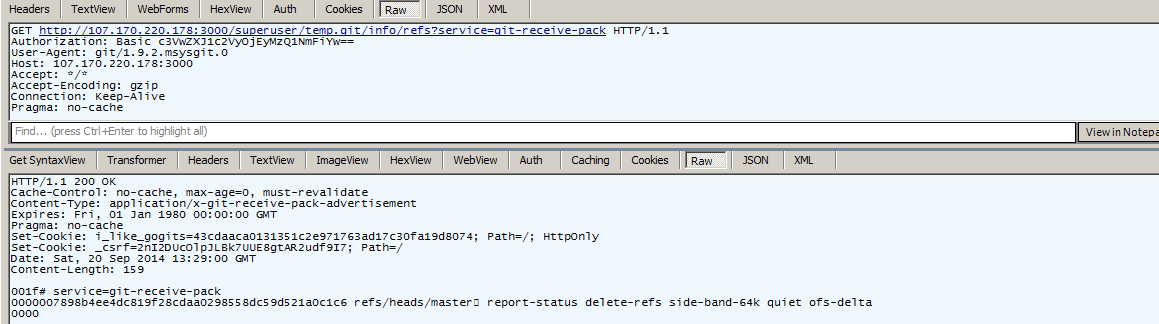
\includegraphics[width=10cm]{git-push-remote-2.png} \\
        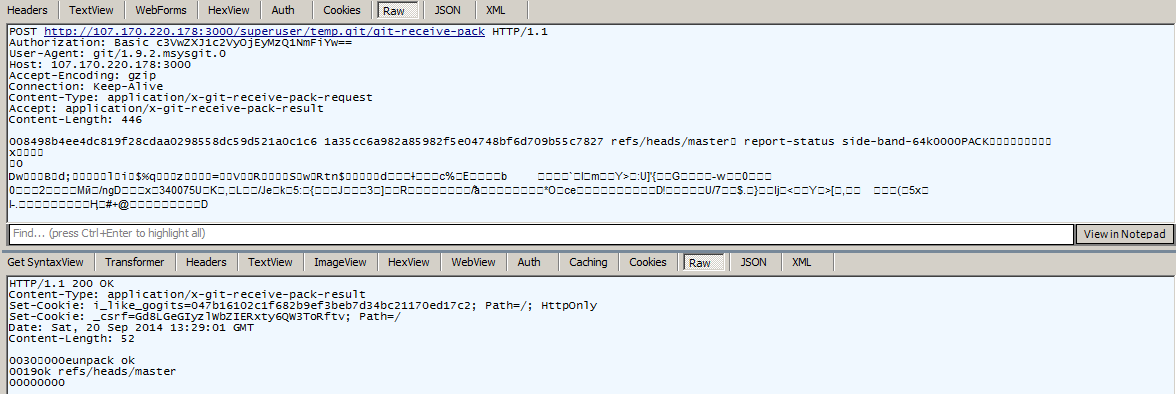
\includegraphics[width=10cm]{git-push-remote-3.png} \\
        git push可能会失败?谁来判定是否失败?
    \end{center}
\end{frame}
\begin{frame}{与远程服务器交互 - git fetch}
    \begin{center}
        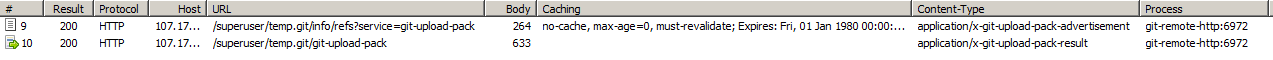
\includegraphics[width=10cm]{git-fetch-remote-1.png} \\
        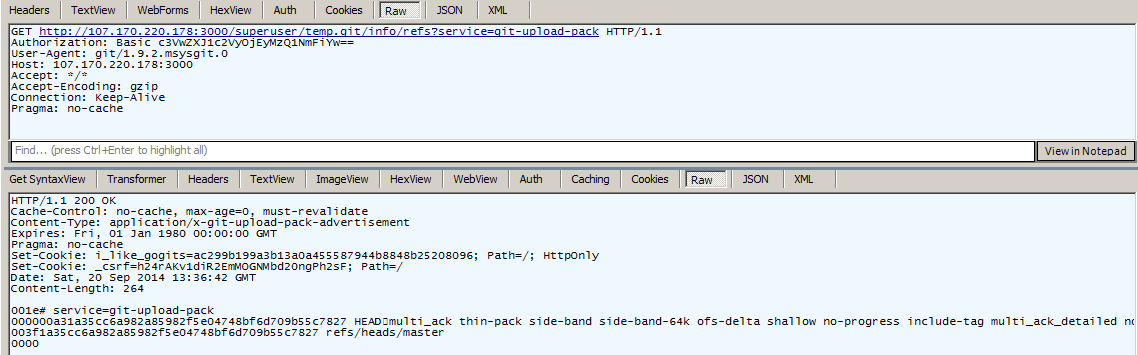
\includegraphics[width=10cm]{git-fetch-remote-2.png} \\
        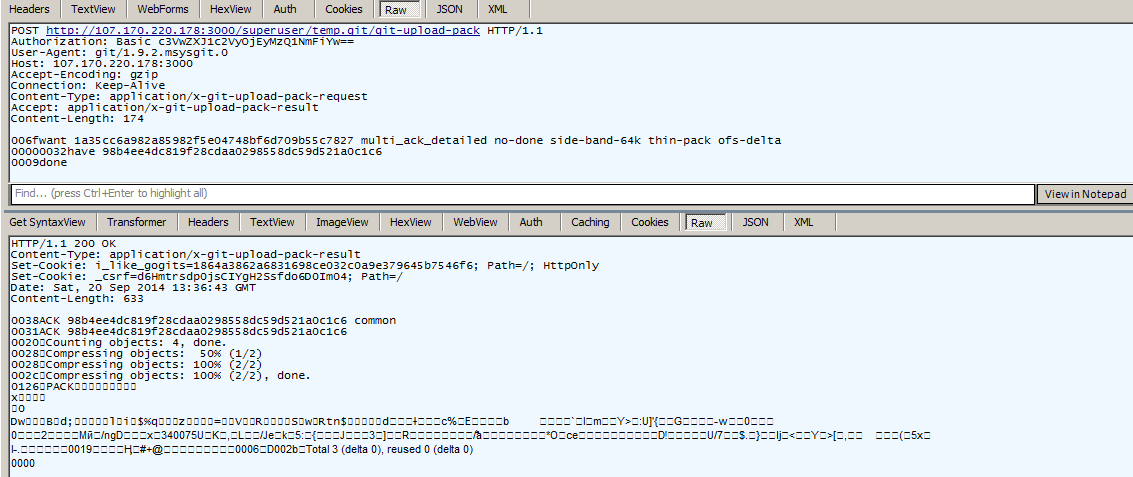
\includegraphics[width=10cm]{git-fetch-remote-3.png}
    \end{center}
\end{frame}

%%%%%%%%%%%%%%%%%%%%%%%%%%%%%%%%
\section{实践(下)}
\begin{frame}{配置}
    \begin{block}{配置文件}
        \begin{itemize}
        \item Git的配置项有三个级别:系统级、用户级、项目级。同一个配置项,后一级覆盖前一级。对应配置文件有三处:
        \begin{itemize}
                \item Linux上,/etc/gitconfig,\$HOME/.gitconfig,.git/config
                \item Windows上,Git安装目录/etc/gitconfig,\$HOME/.gitconfig,.git/config
            \end{itemize}
        \item Git配置修改有两种方式:
        \begin{itemize}
            \item 直接修改配置文件
            \item 使用 git config命令
        \end{itemize}
        \item git config的两个选项--system、--global对应“系统级”和“用户级”,不提供这两个选项则默认为项目级。
        \item 查看配置信息:git config --list,git config user.name
        \end{itemize}
    \end{block}
\end{frame}
\begin{frame}{配置 - 常用配置项}
    \begin{block}{}
        \begin{itemize}
            \item git config --global user.name "John Doe"
            \item git config --global user.email johndoe@example.com
            \item git config --global core.editor d:/softwares/Vim/vim74/gvim.exe
            \item git config --global color.ui true   // 为Git命令输出使用默认着色方案
            \item git config --global http.proxy 127.0.0.1:8087 // HTTP代理
            \item git config --global https.proxy 127.0.0.1:8087 // HTTPS代理
            \item git config --global http.sslVerify false
            \item git config --global http.postBuffer 524288000
        \end{itemize}
    \end{block}
\end{frame}

\begin{frame}{.gitignore}
    \begin{block}{格式规范}
        \begin{itemize}
            \item 所有空行或者以注释符号\#开头的行都会被Git忽略
            \item 可以使用标准的glob模式匹配(所谓的glob模式是指shell所使用的简化了的正则表达式。星号($*$)匹配零个或多个任意字符;
                $[abc]$匹配任何一个列在方括号中的字符问号($?$)只匹配一个任意字符;如果在方括号中使用短划线分隔两个字符,
                表示所有在这两个字符范围内的都可以匹配(比如$[0-9]$表示匹配所有0到9的数字))
            \item 匹配模式最后跟反斜杠(/)说明要忽略的是目录
            \item 要忽略指定模式以外的文件或目录,可以在模式前加上惊叹号($!$)取反
        \end{itemize}
    \end{block}
    \begin{block}{}
    注意:已加入版本控制的文件、目录无法被ignore掉
    
    .gitignore模板集合:\href{https://github.com/github/gitignore}{https://github.com/github/gitignore}
    \end{block}
\end{frame}
\begin{frame}{撤销操作}
    \begin{itemize}
        \item git reset -- files 用来撤销最后一次git add files,你也可以用git reset撤销所有暂存区域文件
        \item git checkout -- files 把文件从暂存区域复制到工作目录,用来丢弃本地修改
    \end{itemize}
    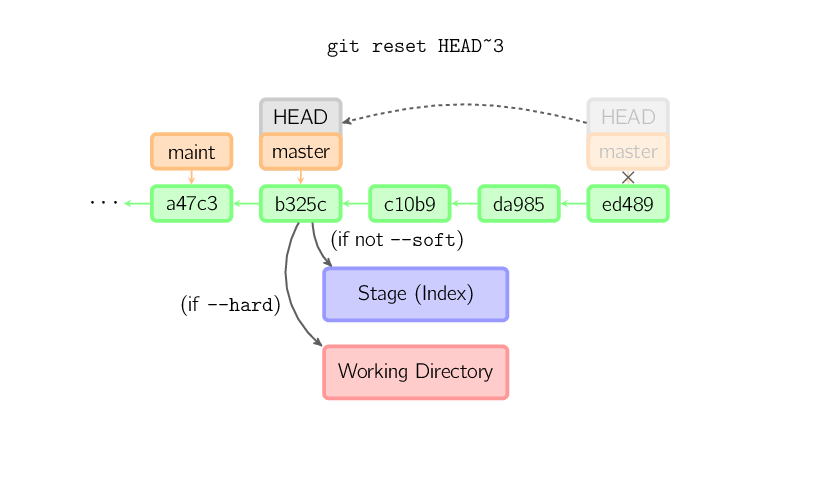
\includegraphics[width=10cm]{reset-commit.png}
\end{frame}
\begin{frame}{分支衍合(rebase)}
    \begin{center}
        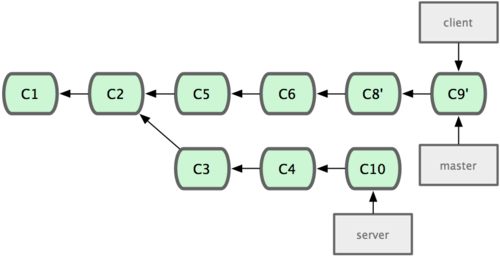
\includegraphics[width=6cm]{git-rebase-1.png} \\
        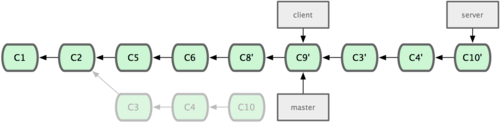
\includegraphics[width=9cm]{git-rebase-2.png}
        \begin{enumerate}
            \item git checkout server
            \item git rebase master
            \item git checkout master
            \item git merge server
        \end{enumerate}
        衍合的优点?问题?
    \end{center}
\end{frame}
\begin{frame}{Stashing}
    \begin{block}{}
        当你正在进行项目中某一部分的工作,里面的东西处于一个比较杂乱的状态,而你想转到其他分支上进行一些工作。问题是,你不想提交进行了一半的工作,
        否则以后你无法回到这个工作点。解决这个问题的办法就是\textbf{git stash}命令。
        \begin{itemize}
            \item git stash /* 对为加入版本控制的文件不起作用,因为分支切换不会影响到这些文件 */
            \item git stash list
            \item git stash apply 
        \end{itemize}
    \end{block}
\end{frame}

\begin{frame}{高级话题}
    \begin{itemize}
        \item 子模块:当你在一个项目上工作时,你需要在其中使用另外一个项目。也许它是一个第三方开发的库或者是你独立开发和并在多个父项目中使用的。
            这个场景下一个常见的问题产生了:你想将两个项目单独处理但是又需要在其中一个中使用另外一个。
        \item 重写历史
        \item git svn
        \item hook
    \end{itemize}
\end{frame}

%%%%%%%%%%%%%%%%%%%%%%%%%%%%%%%%
\section{结束}
\begin{frame}{Git图形化工具推荐}
\begin{itemize}
    \item \href{http://gitextensions.codeplex.com/}{Git Extensions}
    \item \href{https://windows.github.com/}{Github for Windows}
    \item \href{http://www.sourcetreeapp.com/}{SourceTree}
\end{itemize}
\end{frame}
\begin{frame}{参考资料\&推荐阅读}
\begin{itemize}
    \item \href{http://git-scm.com/book/zh}{Pro Git}
    \item \href{http://youngsterxyf.github.io/2013/09/28/learning-git-internals-by-example/}{通过示例学习Git内部构造(译)}
\end{itemize}
\end{frame}

\begin{frame}[plain]
    \begin{center}
        谢谢!
    \end{center}
\end{frame}

\end{CJK*}
\end{document}
